\documentclass[11pt]{article}

\usepackage[utf8]{inputenc}
\usepackage{indentfirst}
\usepackage{natbib}
\usepackage{graphicx}

\renewcommand{\contentsname}{Índice}

\begin{document}

\begin{titlepage}
   \begin{center}
       
       
\includegraphics[width=0.3\textwidth]{images/EscolaEngenhariaUM.jpeg}
       
       \vspace*{0.5cm}
       
       \textbf{\Large Sistema de gestão de stocks de um	armazém de uma fábrica - Fase 2}

       \vspace{1.3cm}
       \textbf{\large Desenvolvimento de Sistemas de Software - Grupo 10}
            
       \vspace{1.3cm}

       Bruno Filipe de Sousa Dias A89583\\ Guilherme Santiago Lopes Pereira A89479 \\ Luís Enes Sousa A89597\\ Pedro Miguel de Soveral Pacheco Barbosa A89529

       \vspace{1.5cm}
       
       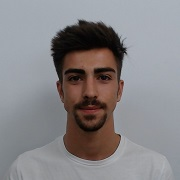
\includegraphics[width=35mm]{images/bruno.jpeg}\hspace{0.2cm}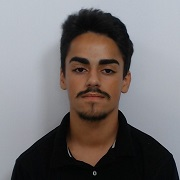
\includegraphics[width=35mm]{images/guilherme.jpeg}
       \vspace{0.15cm}
       \hspace{0.1cm}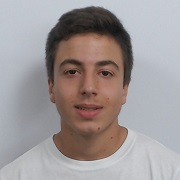
\includegraphics[width=35mm]{images/luis.jpeg}\hspace{0.1cm}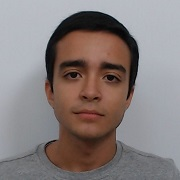
\includegraphics[width=35mm]{images/pedro.jpeg}
       
        
        28 de novembro de 2020
            
   \end{center}
\end{titlepage}

\tableofcontents
\thispagestyle{empty}
\cleardoublepage

\setcounter{page}{1}

\section{Introdução}

Neste semestre, no âmbito da unidade curricular de Desenvolvimento de Sistemas de Software, foi-nos proposto o desenvolvimento de uma componente de um sistema de gestão de stocks de um armazém de uma fábrica de modo a pôr em prática toda a aprendizagem sobre Desenvolvimento de Sistemos de Software, com auxílio da linguagem de programação orientada aos objetos Java. O seu principal objetivo será desenvolver uma aplicação que suporte alguns cenários descritos no enunciado pelos docentes da cadeira e outros que serão definidos pelo nosso grupo consoante achemos pertinente ao longo da realização deste projeto.

O trabalho foi dividido em três fases de entrega sendo que a segunda consiste na modelação concetual da solução que será feita com base na conceção de Diagramas de Sequência, Diagrama de Classes, Diagrama de Componentes e Diagrama de Packages.

\section{Diagrama de Classes}

Após a conceção do Modelo de Domínio e dos diversos Use Cases na 1ª fase do nosso projeto foi necessário construir um Diagrama de Classes para perceber quais são as entidades mais relevantes do nosso trabalho e perceber a maneira como estas se relacionam entre si. Assim, o nosso grupo construiu o seguinte Diagrama de Classes:

\begin{figure}[htb]
    \centering
    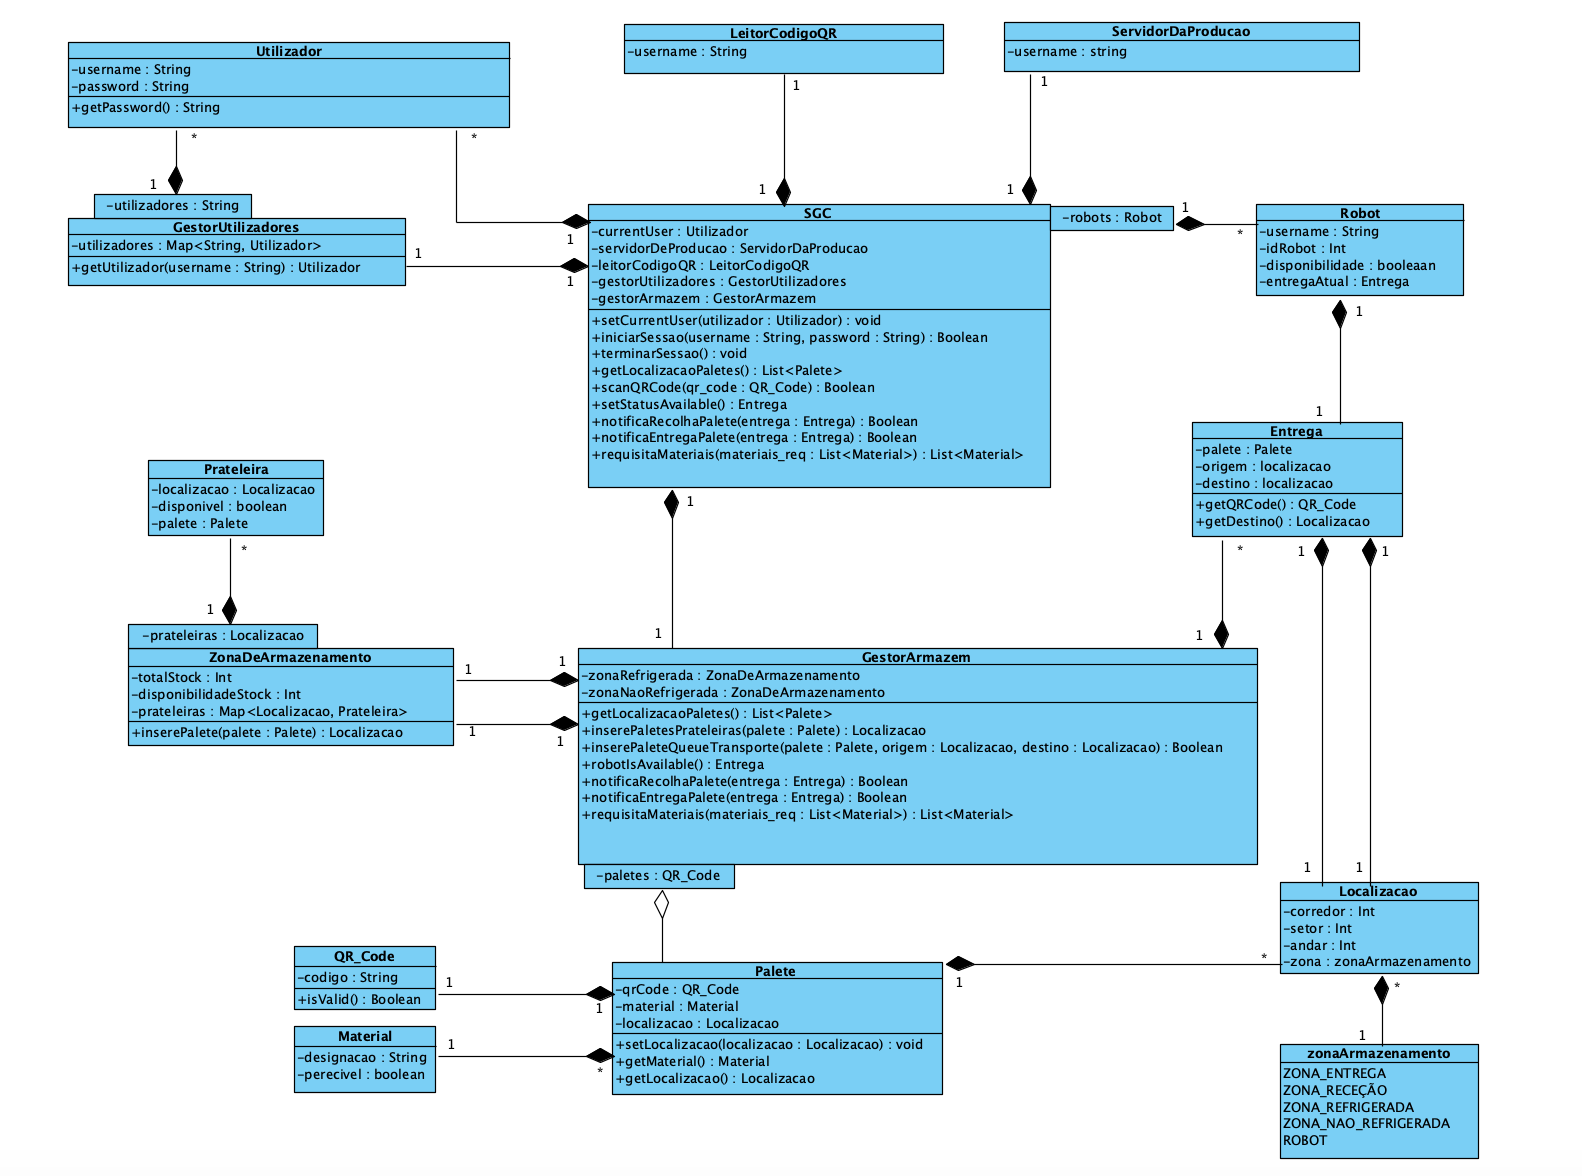
\includegraphics[width=1\textwidth]{images/diagramaclasses.png}
    \caption{Diagrama de Classes}
    \label{fig:my_label3}
\end{figure}

\clearpage

\section{Diagramas de Sequência}

Nesta parte do projeto, serão apresentados todos os Diagramas de Sequência elaborados a partir das especificações dos diferentes Use Cases. Desta forma, o objetivo é apresentar todas as operações fundamentais para o correto funcionamento da nossa aplicação.

\subsection{Ator : Gestor}

\subsubsection{Consultar Listagens de Localização}

\begin{figure}[htb]
    \centering
    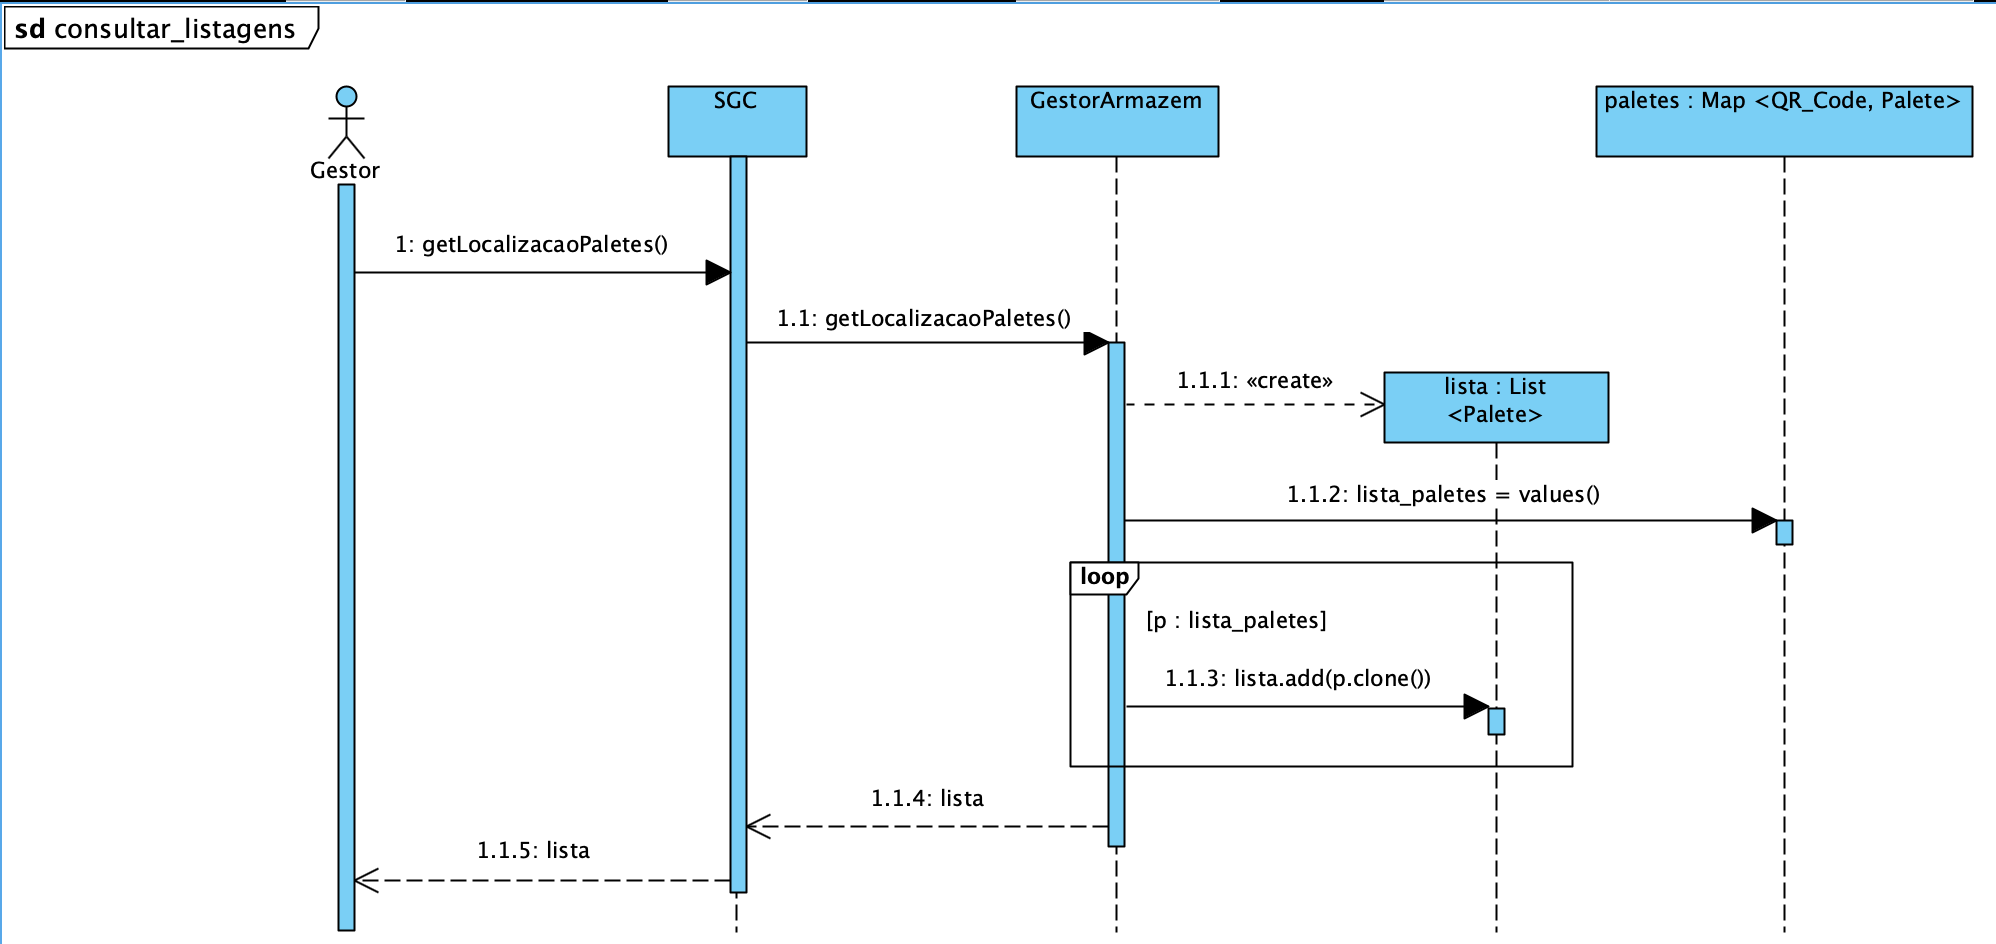
\includegraphics[width=0.9\textwidth]{images/consultarlistagens.png}
    \caption{Diagrama de Sequência - Consultar Listagens de Localização}
    \label{fig:my_label1}
\end{figure}

\clearpage

\subsubsection{Iniciar Sessão}

\begin{figure}[htb]
    \centering
    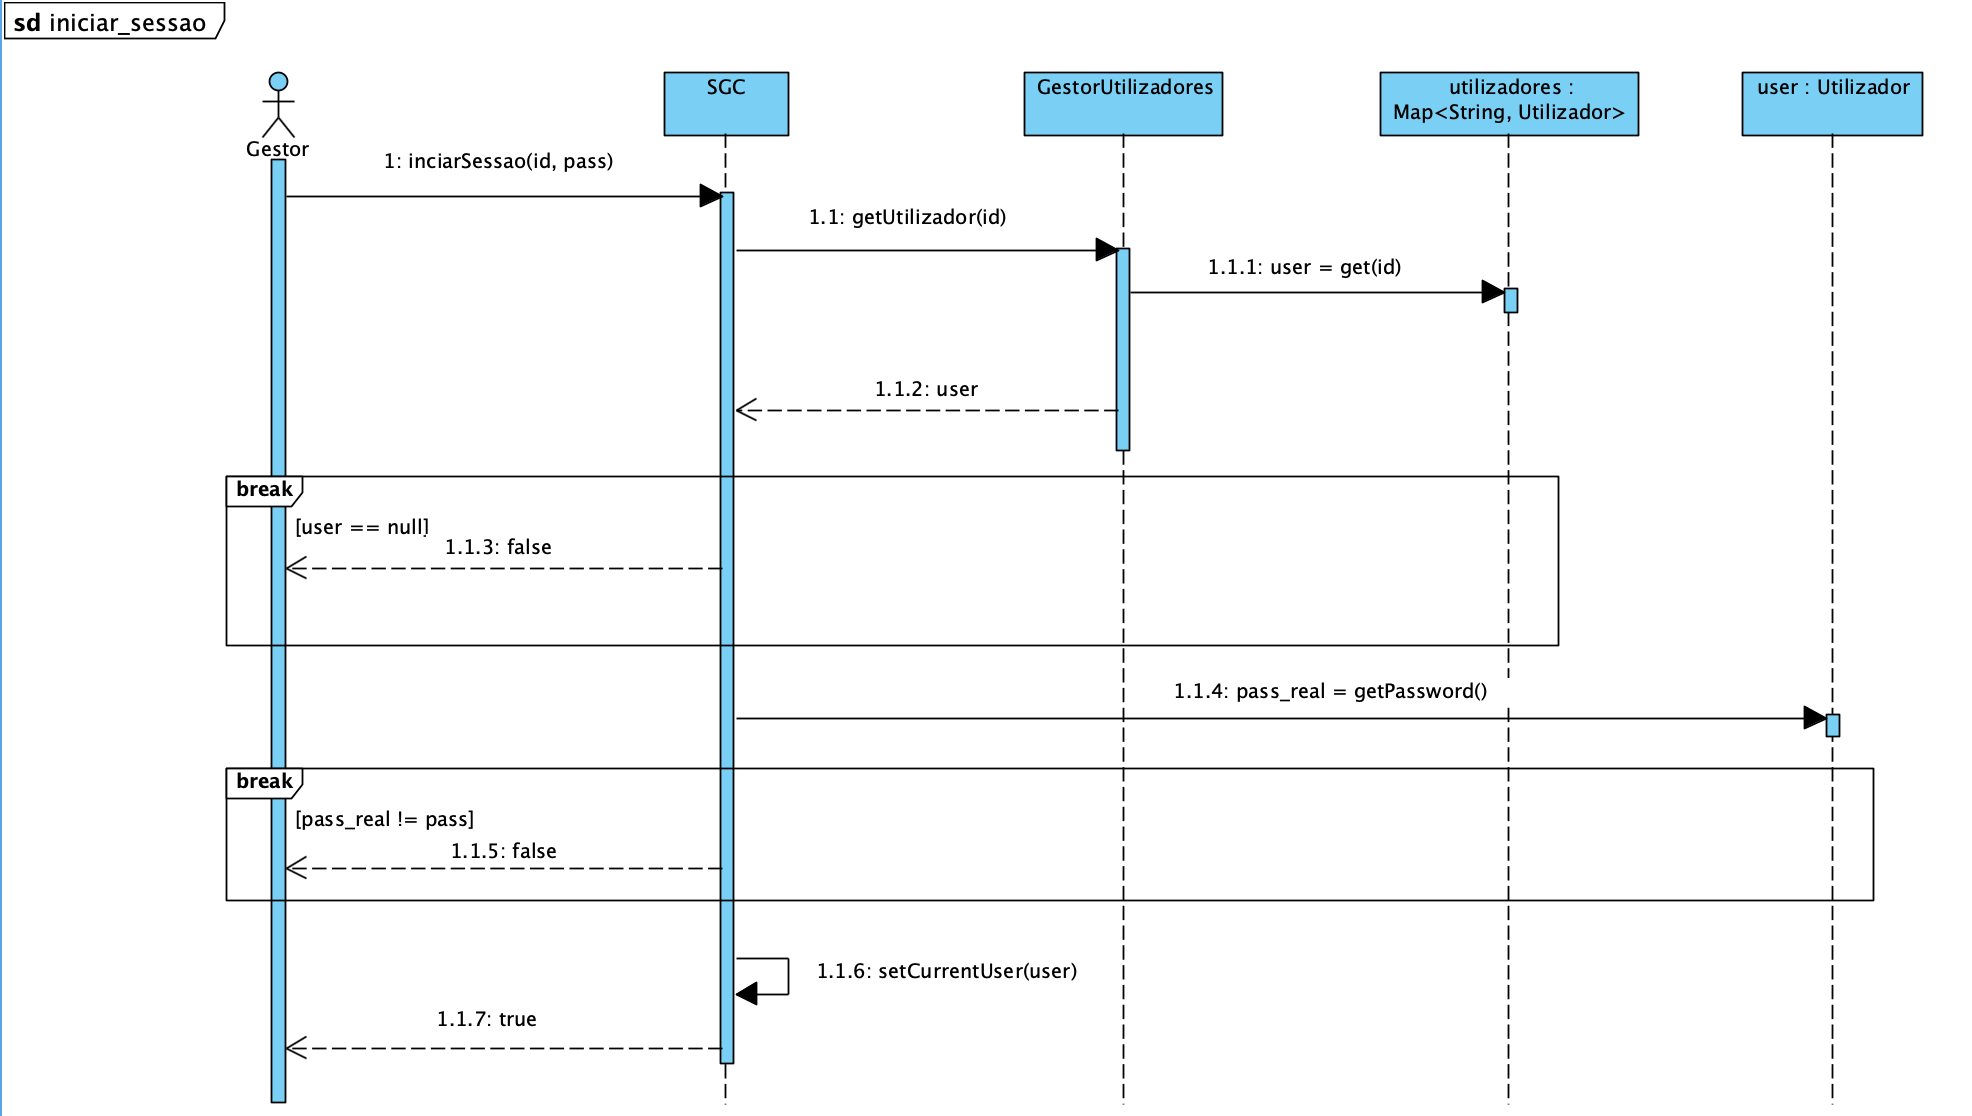
\includegraphics[width=0.9\textwidth]{images/iniciarsessao.png}
    \caption{Diagrama de Sequência - Iniciar Sessão}
    \label{fig:my_label2}
\end{figure}

\subsubsection{Terminar Sessão}

\begin{figure}[htb]
    \centering
    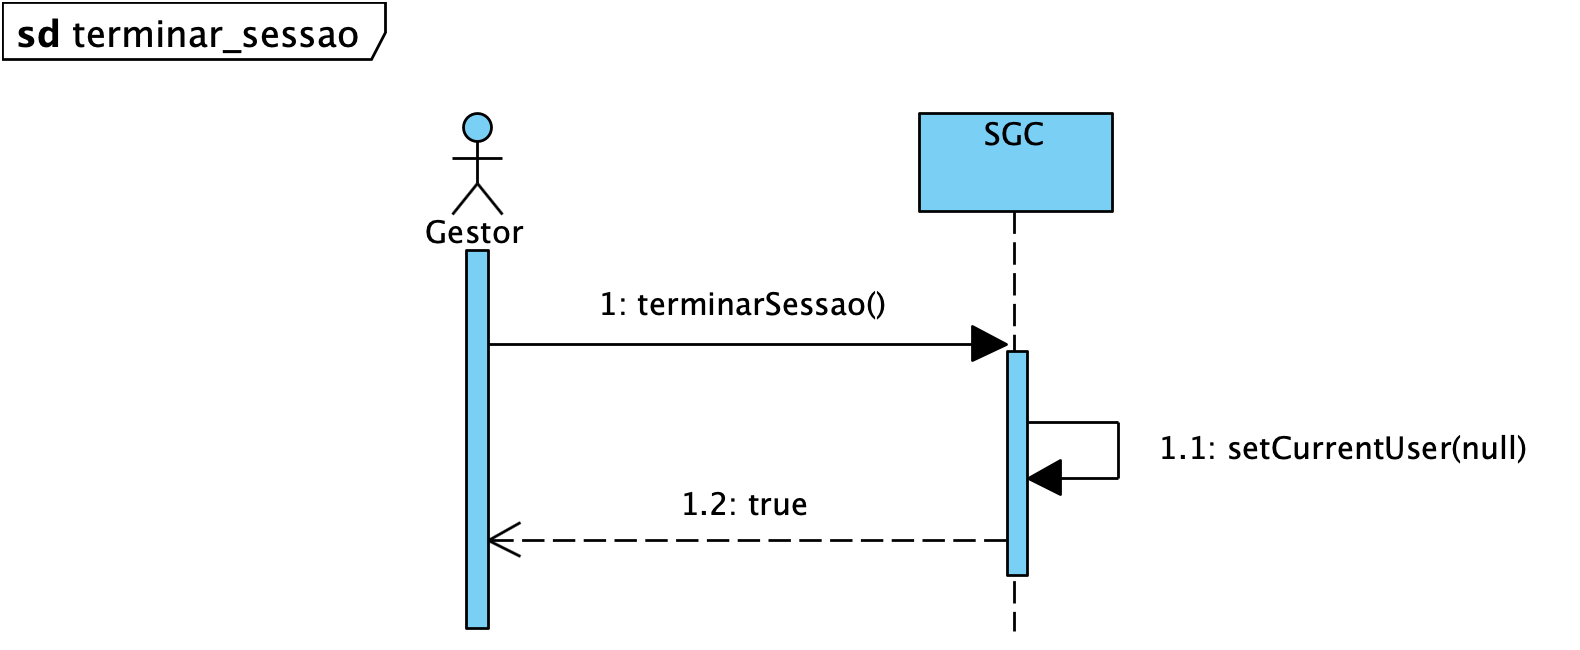
\includegraphics[width=1\textwidth]{images/terminarsessao.png}
    \caption{Diagrama de Sequência - Terminar Sessão}
    \label{fig:my_label3}
\end{figure}

\clearpage

\subsection{Ator : Leitor de Códigos QR}

\subsubsection{Comunicar Código QR}

\begin{figure}[htb]
    \centering
    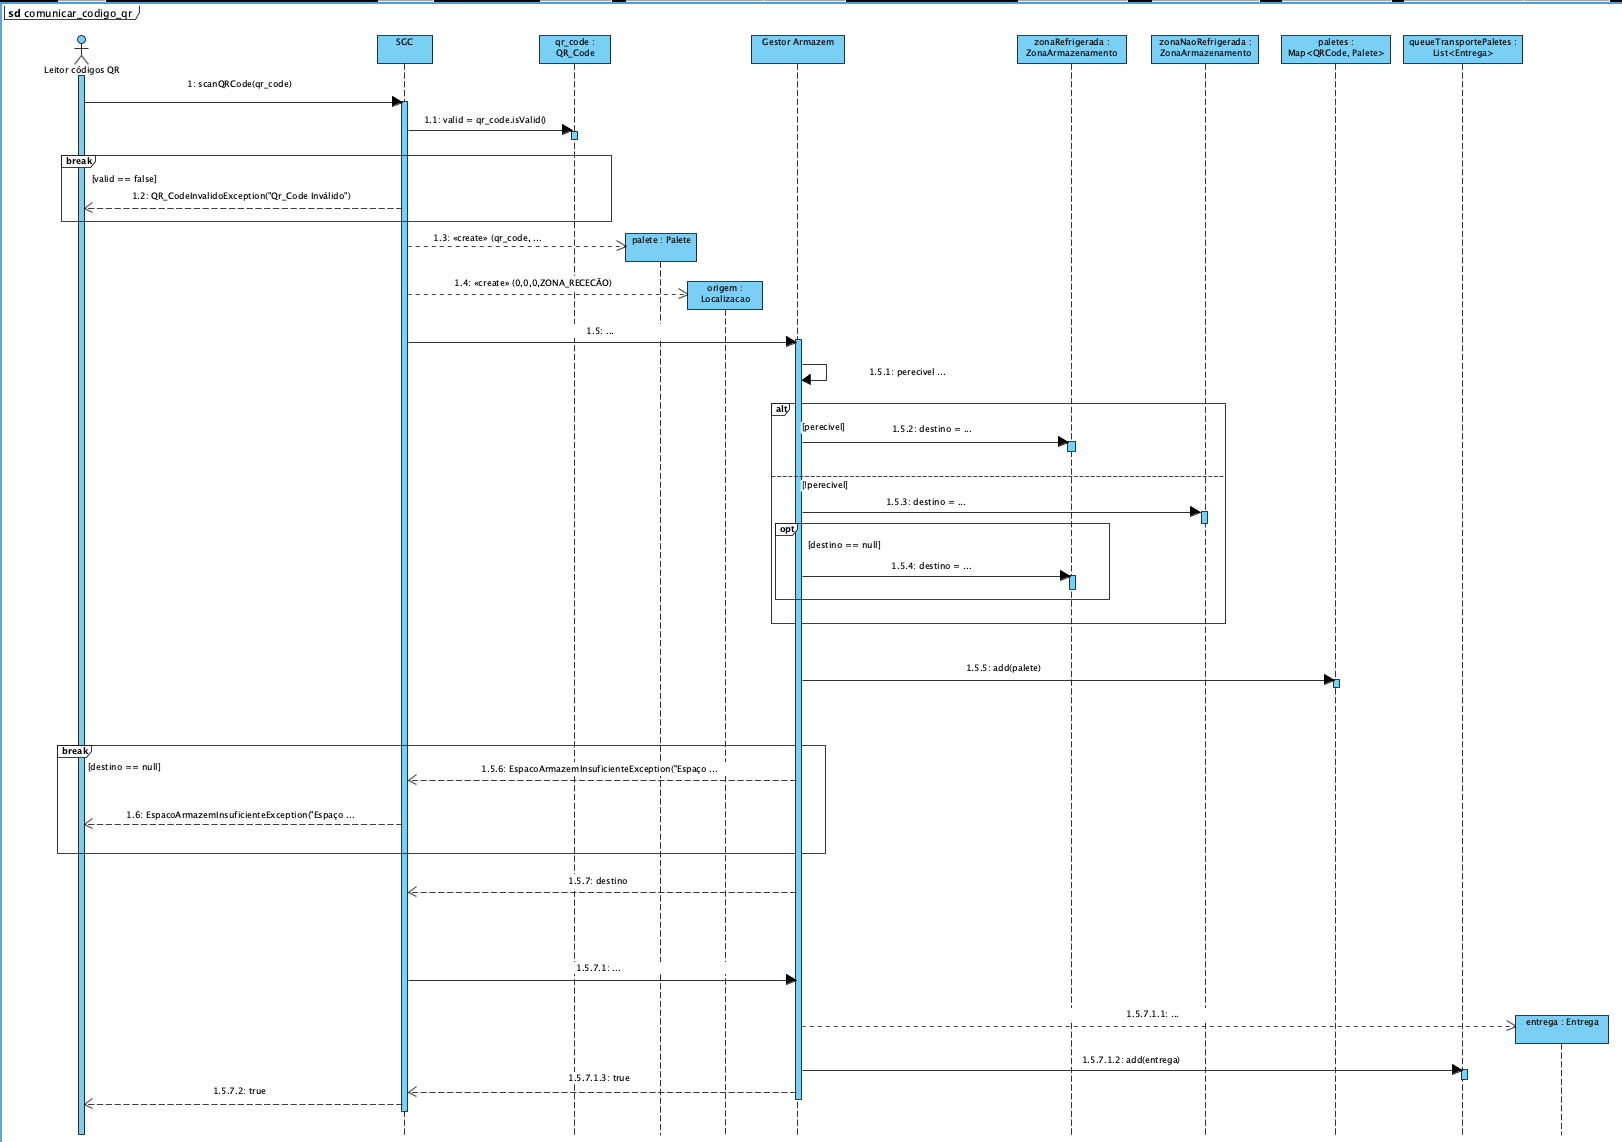
\includegraphics[width=1\textwidth]{images/comunicarcodigoqr.png}
    \caption{Diagrama de Sequência - Comunicar Código QR}
    \label{fig:my_label3}
\end{figure}

\clearpage

\subsection{Ator : Robot}

\subsubsection{Sistema Comunica Ordem de Transporte}

\begin{figure}[htb]
    \centering
    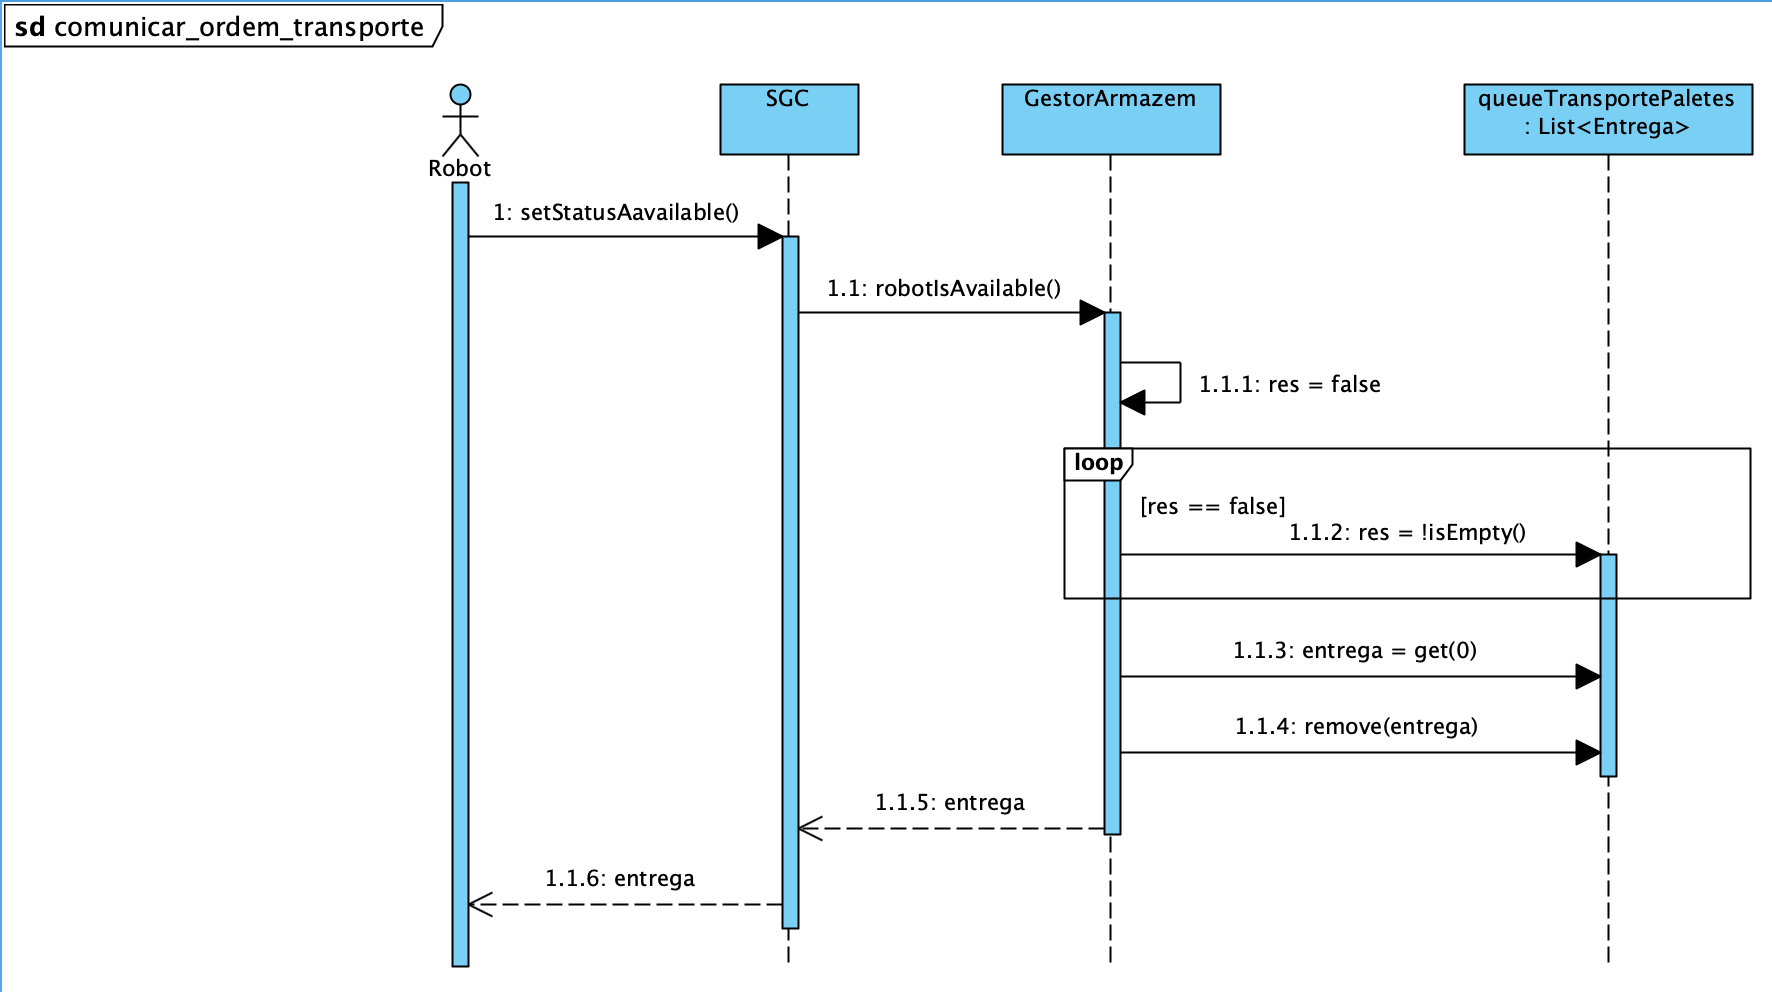
\includegraphics[width=1\textwidth]{images/comunicarordemtransporte.png}
    \caption{Diagrama de Sequência - Comunicar Ordem de Transporte}
    \label{fig:my_label3}
\end{figure}

\subsubsection{Notificar Recolha de Paletes}

\begin{figure}[htb]
    \centering
    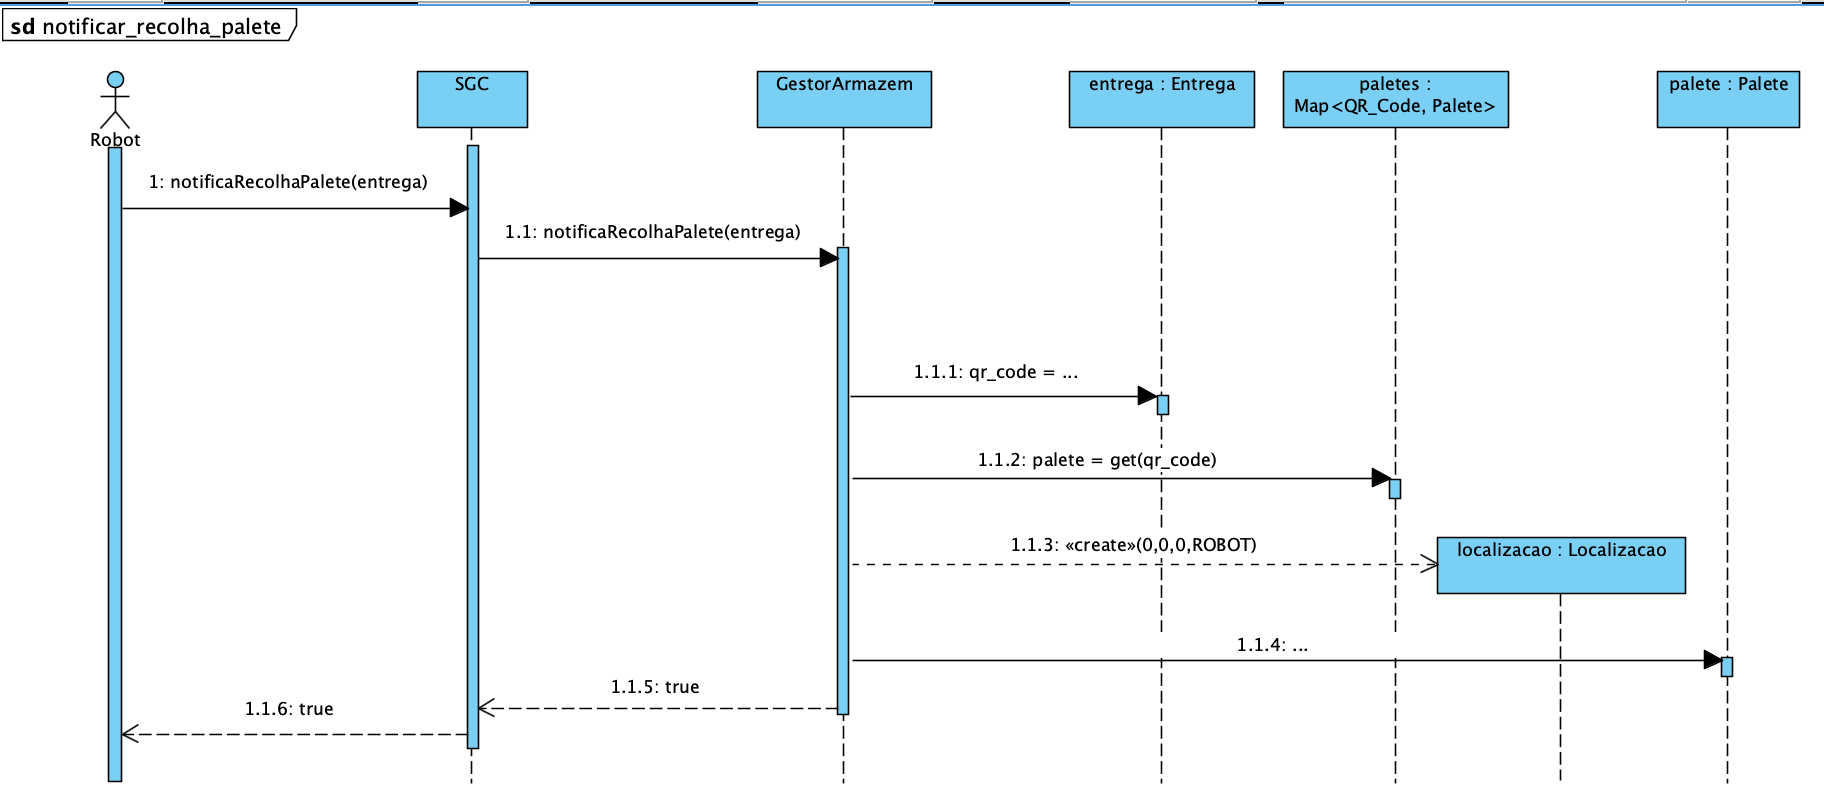
\includegraphics[width=0.8\textwidth]{images/notificarrecolhapalete.png}
    \caption{Diagrama de Sequência - Notificar Recolha Palete}
    \label{fig:my_label3}
\end{figure}

\clearpage

\subsubsection{Notificar Entrega de Paletes}

\begin{figure}[htb]
    \centering
    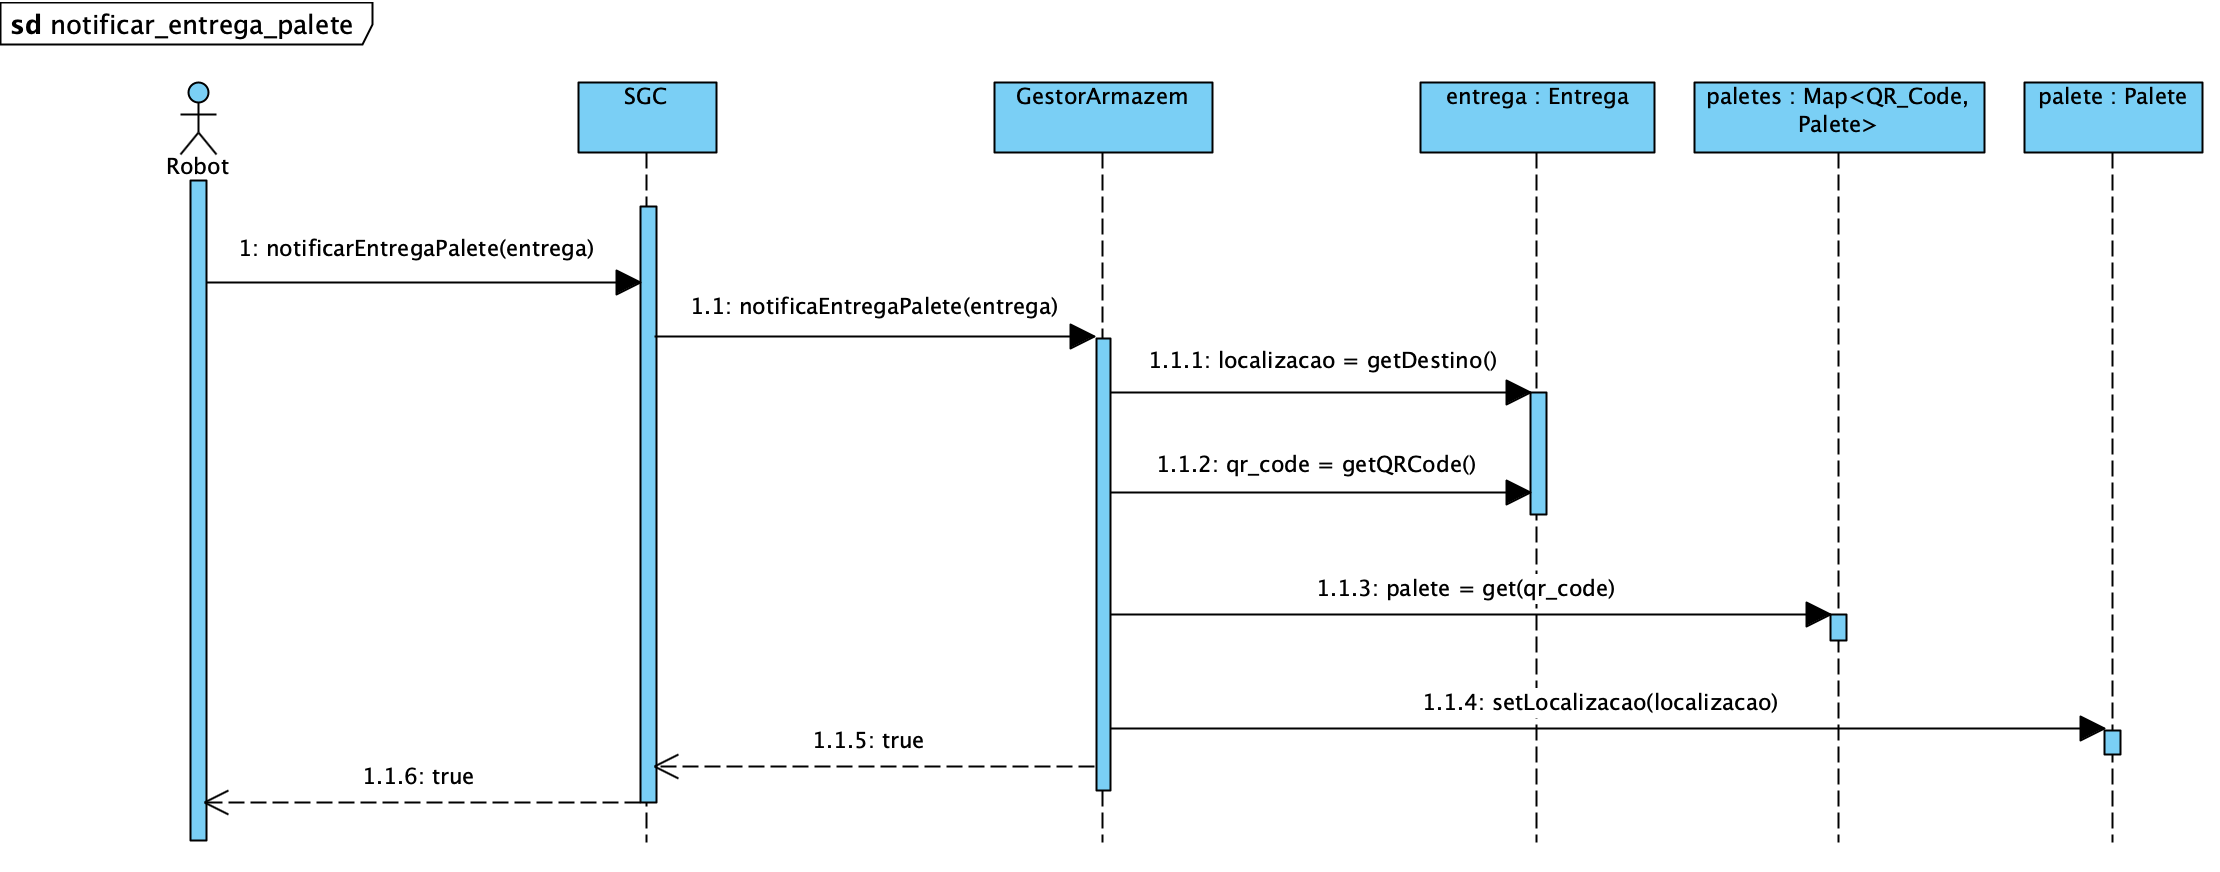
\includegraphics[width=1\textwidth]{images/notificarentregapalete.png}
    \caption{Diagrama de Sequência - Notificar Entrega Palete}
    \label{fig:my_label3}
\end{figure}

\clearpage

\subsection{Ator : Servidor da Produção}

\subsubsection{Requisitar Paletes}

\begin{figure}[htb]
    \centering
    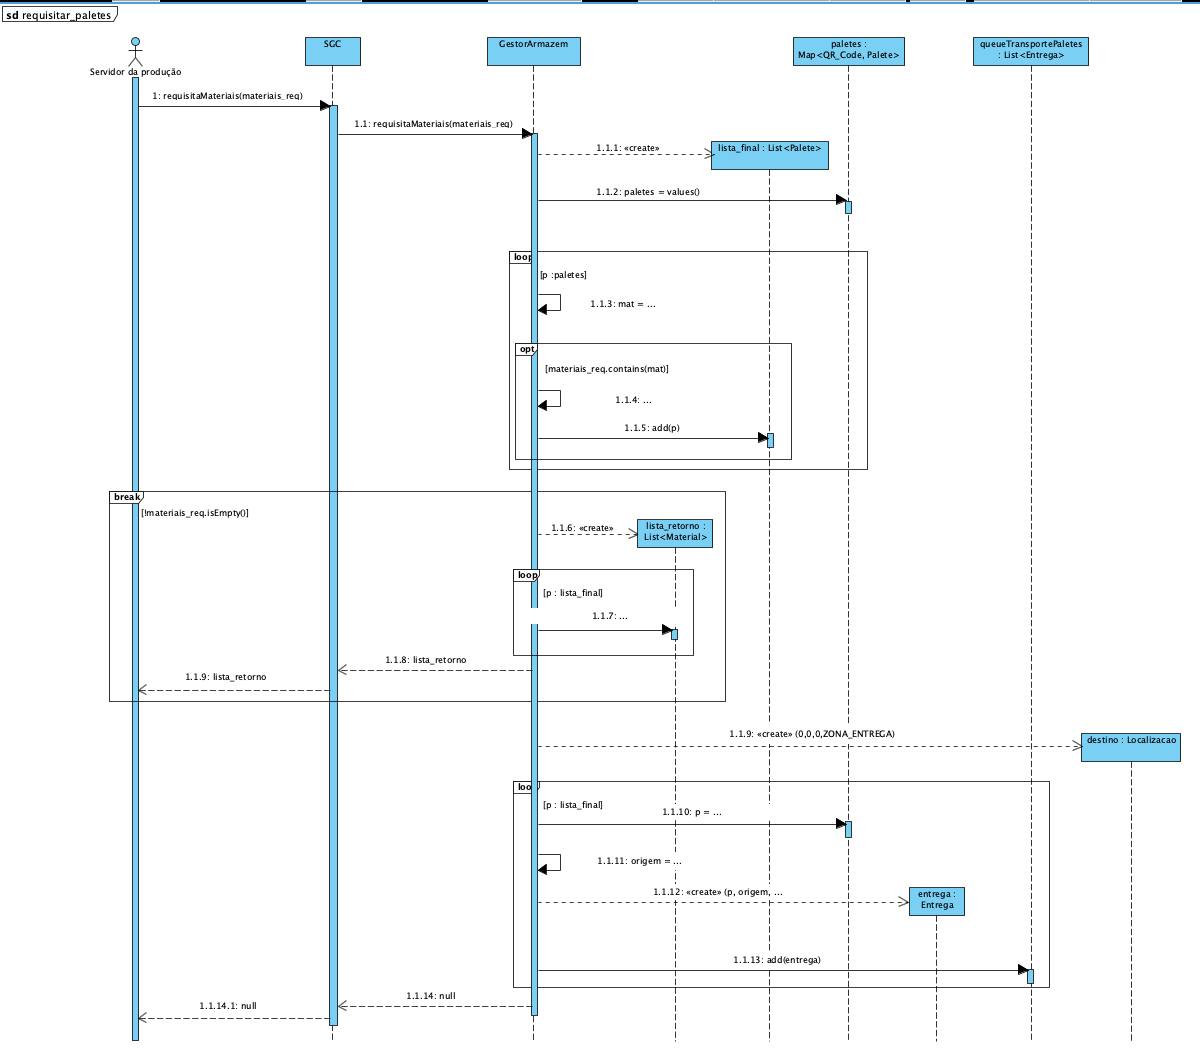
\includegraphics[width=1\textwidth]{images/requisitarpaletes.png}
    \caption{Diagrama de Sequência - Requisitar Paletes}
    \label{fig:my_label3}
\end{figure}

\clearpage

\section{Diagrama de Packages}

De seguida apresentamos o nosso Diagrama de Packages onde é possível verificar como é que o nosso grupo procedeu à divisão lógica do projeto.

\begin{figure}[htb]
    \centering
    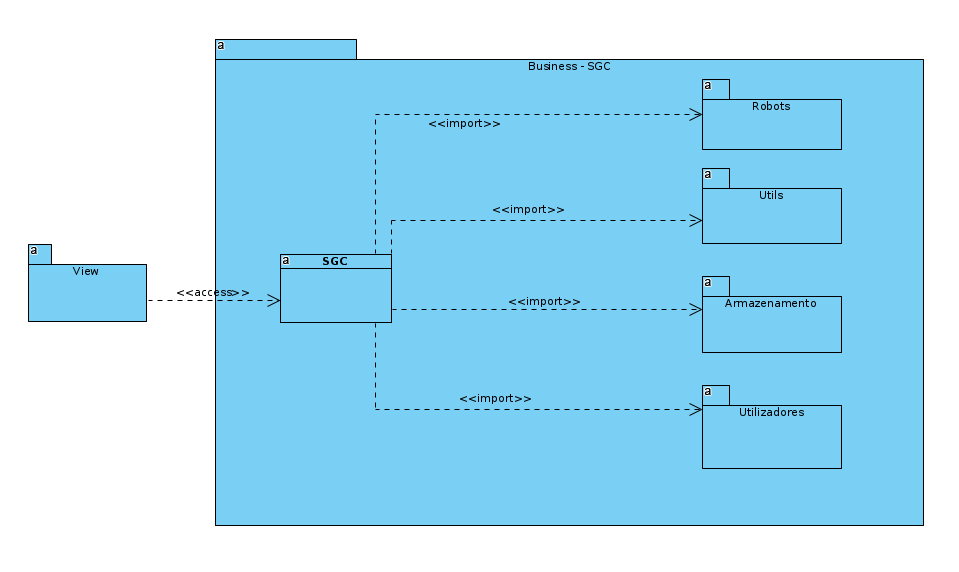
\includegraphics[width=1\textwidth]{images/diagramapackages.png}
    \caption{Diagrama de Packages}
    \label{fig:my_label3}
\end{figure}

\clearpage

\section{Diagrama de Componentes}

\begin{figure}[htb]
    \centering
    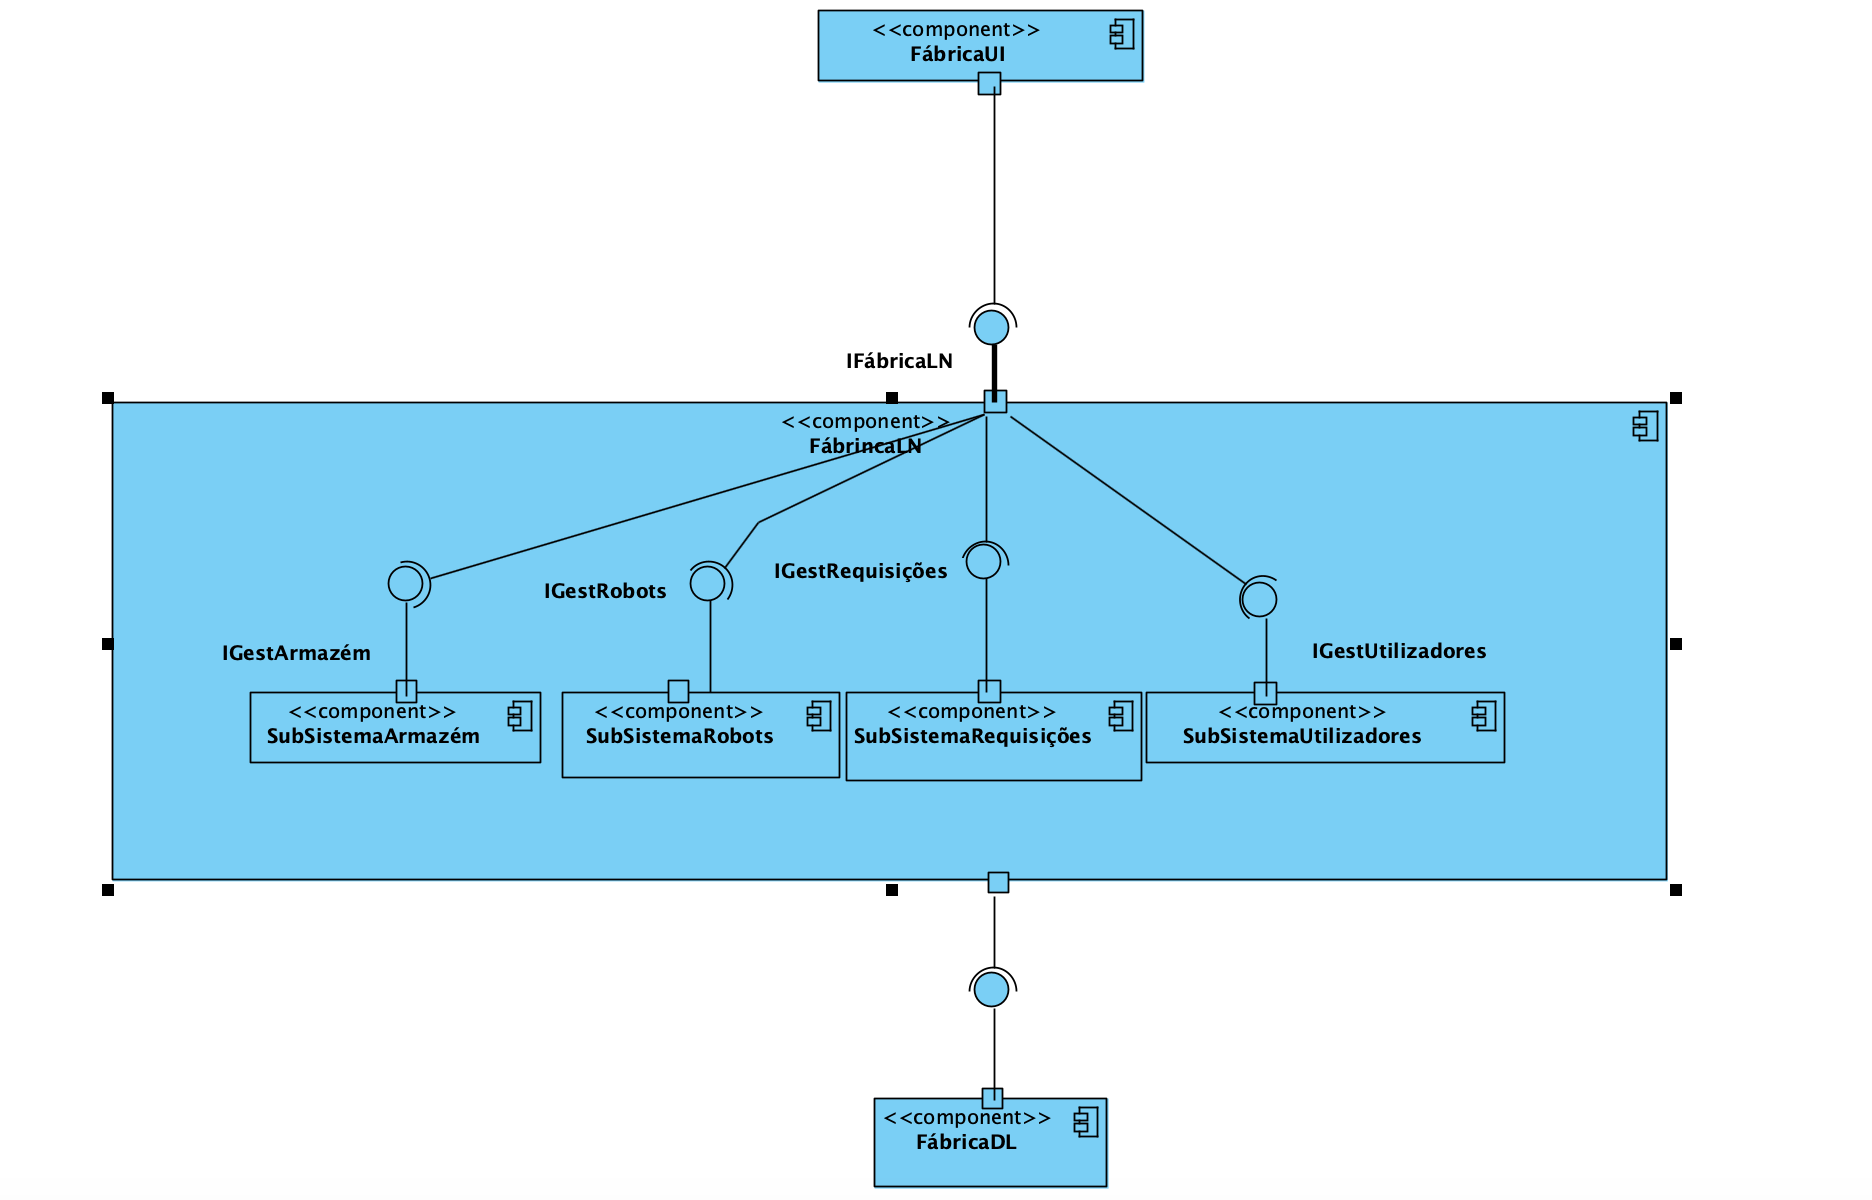
\includegraphics[width=1\textwidth]{images/diagramacomponentes.png}
    \caption{Diagrama de Componentes}
    \label{fig:my_label3}
\end{figure}

\clearpage

\section{Conclusão}

Concluindo, nesta fase do projeto foi-nos pedido a modelação concetual da solução e prosseguimos à elaboração dos Diagramas de classe, de sequência, de componentes e de packages. Todo este processo permitiu o grupo ter uma melhor perceção da maneira como as entidades relevantes se relacionam entre si. Seguidamente, através dos Diagramas de Sequência, percebemos o comportamento dos diferentes Use Cases do nosso projeto e como se processa a sequência de processos nos mesmos. Deste modo, pensamos que atingimos o nosso objetivo que consistia em perceber através da modelação concetual da solução como é que iriam funcionar todos os processos de gerir o stock da fábrica com foco tanto nas entidades existentes como na maneira como estas se vão relacionar entre si. Esperamos assim ter conseguido, através da elaboração da 2ª fase do projeto, ter atingido todos os objetivos que nos permitam construir uma aplicação o mais eficiente e completa possível.

\end{document}



